\chapter{Background}
\label{chapter:background}

\section{Ethereum Smart Contract}

\newpage
\section{MetaMask}
Metamask is a chrome extension for accessing Ethereum distributed application (DApp), this extension can enable web3 API in website so that users can interact with any Etehereum blockchain from Javascript~\cite{web3.js}, e.g., Mainnet, Testnet. It also creates identities by the user themself. The user of Metamask can create and manage their identities; moreover, Metamask provides an interface that user can perform a transaction to the connected blockchain.\par
Because the user manages owned Ethereum account through Metamask, the user can use their private key to sign a transaction or sign data to prove ownership of an account.\par


\begin{figure}[hb]
    \centering
    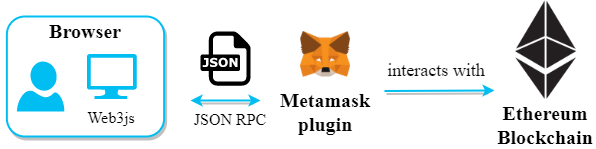
\includegraphics[height=!,width=1\linewidth,keepaspectratio=true]{figures/architecture_of_dapp.png}
    \caption{{\footnotesize Architecture of Dapp}}
    \label{fig:architecture_of_dapp}
\end{figure}

\section{ECDSA}
\newpage
\section{OAuth}

\section{Trust Service Provider (TSP)}

\section{Related work}
